\documentclass{standalone}
\usepackage{graphicx}	
\usepackage{amssymb, amsmath}
\usepackage{color}

\usepackage{tikz}
\usetikzlibrary{intersections, backgrounds, math, decorations.pathreplacing}
\usepackage{pgfmath}

\definecolor{light}{RGB}{220, 188, 188}
\definecolor{mid}{RGB}{185, 124, 124}
\definecolor{dark}{RGB}{143, 39, 39}
\definecolor{highlight}{RGB}{180, 31, 180}
\definecolor{light_teal}{RGB}{107, 142, 142}
\definecolor{mid_teal}{RGB}{72, 117, 117}
\definecolor{dark_teal}{RGB}{29, 79, 79}
\definecolor{gray10}{gray}{0.1}
\definecolor{gray20}{gray}{0.2}
\definecolor{gray30}{gray}{0.3}
\definecolor{gray40}{gray}{0.4}
\definecolor{gray50}{gray}{0.5}
\definecolor{gray60}{gray}{0.6}
\definecolor{gray70}{gray}{0.7}
\definecolor{gray80}{gray}{0.8}
\definecolor{gray90}{gray}{0.9}
\definecolor{gray95}{gray}{0.95}

\begin{document}

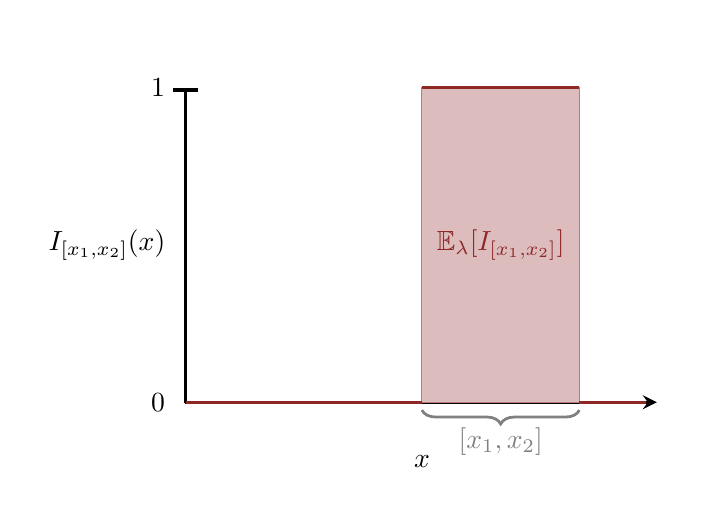
\begin{tikzpicture}[scale=1.0]

  \draw[white] (-5, -3.25) rectangle (3.5, 2.75);
  
  \draw [-|, >=stealth, line width=1.25] (-3.00, -2.015) -- +(0, 4);
  \draw [->, >=stealth, line width=1.25] (-3.015, -2.00) -- +(6, 0);
  
  \filldraw[fill=light, draw=mid] (0, -2) rectangle (2, 2);
  \node[dark] at (1, 0) { $\mathbb{E}_{\lambda} [ I_{[x_{1}, x_{2}]} ]$ }; 
  
  \draw[dark, line width = 1.25] (-3, -2) -- (0, -2);
  \draw[dark, line width = 1.25] (0, +2) -- (2, 2);
  \draw[dark, line width = 1.25] (2, -2) -- (2.85, -2);
  
  \draw[gray50, line width=1, decorate,decoration={brace,amplitude=5pt,mirror}] (0, -2.1) -- (2, -2.1);
  \node[gray50] at (1, -2.5) { $[x_{1}, x_{2}]$ };
  
  \node at (-3.35, -2) { $0$ };
  \node at (-3.35, +2) { $1$ };
  \node at (-4, 0) { $I_{[x_{1}, x_{2}]}(x)$ };
  
  
  \node at (0, -2.75) { $x$ };

  
\end{tikzpicture}

\end{document}  